\documentclass[12pt]{article}
\usepackage[left = 0.6in, right = 0.6in, top = 0.4in, bottom = 1.5in]{geometry} 
\usepackage{listings, pgfplots, fontawesome5, booktabs, xcolor, hyperref, amsmath,amsthm,amssymb,amsfonts, enumitem, fancyhdr, color, comment, graphicx, environ, actuarialsymbol}
\usepackage[dvipsnames]{xcolor}
\pagestyle{fancy}
\setlength{\headheight}{65pt}
%%%%%%%%%%%%%%%%%%%%%%%%%%%%%%%%%%%%%%%%%%%%%
\lhead{}
\rhead{rational functions and addition of ordinates}
%%%%%%%%%%%%%%%%%%%%%%%%%%%%%%%%%%%%%%%%%%%%%
\newcommand{\emptygrid}[3]{ % #1: range, #2: y-label, #3: "labels" or "nolabels"
    \begin{tikzpicture}
    \begin{axis}[
        axis lines = middle,
        xlabel = $x$,
        ylabel = $#2$,
        xmin=-#1, xmax=#1,
        ymin=-#1, ymax=#1,
        grid = both,
        grid style = {line width=.1pt, draw=gray!30},
        xtick distance = 5,
        ytick distance = 5,
        minor tick num = 4,
        tick label style = {font=\tiny},
        width=10cm, height=10cm,
        axis equal image,
        % Logic to hide labels if #3 is "nolabels"
        xticklabels={ \ifx\empty#3\empty\else\ifnum\pdfstrcmp{#3}{nolabels}=0 \else \fi\fi },
        yticklabels={ \ifx\empty#3\empty\else\ifnum\pdfstrcmp{#3}{nolabels}=0 \else \fi\fi }
    ]
    \end{axis}
    \end{tikzpicture}
}
%%%%%%%%%%%%%%%%%%%%%%%%%%%%%%%%%%%%%%%%%%%%%
\newtheorem{theorem}{Theorem}[section]
\begin{document}


\section{Addition of ordinates review}

adding $y$-values for a given $x$-value

    Consider graphing $f: (0 , 2\pi ) \to \mathbb{R}, f(x) = \frac{x^{2}}{10} + \sin(x)$

    \begin{center}
    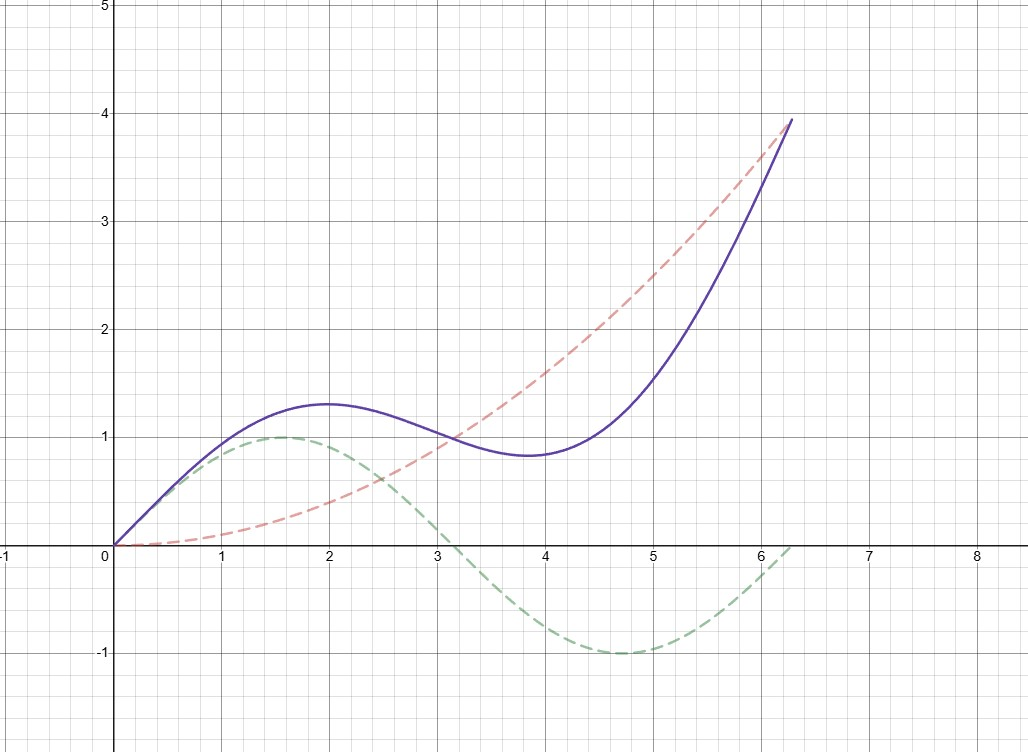
\includegraphics[scale = 0.5]{img1.jpg}
    \end{center}

strategy?
\begin{itemize}
    \item start with finding key points of each curve (if there are any)
    \item plot the curves individually
    \item add the height of each curve at discrete intervals (i.e at every tick )
    \item make sure the y values at key points match
\end{itemize}

New way to think of dilation from the y axis! i.e : $f(x) = 2x^{2} = x^{2} + x^{2}$
\newpage
\section{Rational functions}
\begin{enumerate}

\item $g: \mathbb{R} \to \mathbb{R}, g(x) = \frac{1+x^{2}}{x}$

\begin{center}
\emptygrid{10}{g}{label}
\end{center}

\item $g: \mathbb{R}^{+} \to \mathbb{R}, g(x) = \frac{1+x^{\frac{5}{2}}}{x^{2}}$

\begin{center}
\emptygrid{10}{g}{label}
\end{center}

\newpage

\item ($\ddagger$) $g: \mathbb{R}^{} \to \mathbb{R}, g(x) = \frac{x^{2}|x|-2x^{2} + 1}{|x|} $

\begin{center}
\emptygrid{10}{g}{label}
\end{center}

Trick with plotting graphs with modulus functions: Remember the effects of:
\begin{itemize}
    \item $f(| x |)$
    \item $| f(x) |$
\end{itemize}




\end{enumerate}

\section{Asymptotes}
Types of asymptotes:
\begin{itemize}
    \item Vertical asymptotes : occur when the function approaches infinity as $x$ approaches a certain value
    \begin{itemize}
        \item often occur at values that \textbf{make the denominator zero} 
    \end{itemize}
    \item Horizontal asymptotes : occur when the function approaches a constant value as $x \to \infty$
    \item Oblique asymptotes : occur when the function approaches a linear function as $x \to \infty$
\end{itemize}

Which asymptotes can they cross?
\begin{itemize}
    \item Vertical asymptotes : never, \textbf{because if denom = 0 then function is undefined}
    \item Horizontal asymptotes : can cross
    \item Oblique asymptotes : can cross
\end{itemize}
\newpage

Try to find the asymptotes of the following functions by hand, then use mathematica to verify (plot + calculate limit if needed)
\begin{itemize}
    \item $y = \frac{2x+3}{x-1}$
    \item $y = \frac{x}{x^{2}+1}$
    \item $y = \frac{2x^{3} + x^{2} + x}{ x^{2} - 9}$
\end{itemize}


\section{Useful mathematica code}
\begin{itemize}
    \item Plotting: (This will be the most used function in both methods and spesh, memorise it!)

\texttt{Plot[<expr>, \{x, <xmin>, <xmax>\}, PlotRange -> \{<ymin>,<ymax>\}]}

    \item Plotting multiple functions:

\texttt{Plot[\{<expr1>, <expr2>, <expr3>\}, \{x, <xmin>, <xmax>\}, PlotRange -> \{<ymin>,<ymax>\}]}

    \item Calculating limits:

\texttt{Limit[<expr>, x -> <val>] }


\end{itemize}


\end{document}